%%%%%%%%%%%%%%%%%%%%%%%%%%%%%%%%%%%%%%%%%%%%%%%%%%%%%%%%%%%%%%%%%%%%%%%%%%%%%%%%
% Set Clock
%%%%%%%%%%%%%%%%%%%%%%%%%%%%%%%%%%%%%%%%%%%%%%%%%%%%%%%%%%%%%%%%%%%%%%%%%%%%%%%%
\chapter{Set Clock} \label{Set Clock}
\vspace{-10ex}\mSC{syml}\vskip 8ex

%%%%%%%%%%%%%%%%%%%%%%%%%%%%%%%%%%%%%%%%%%%%%%%%%%%%%%%%%%%%%%%%%%%%%%%%%%%%%%%%
% Introduction
%%%%%%%%%%%%%%%%%%%%%%%%%%%%%%%%%%%%%%%%%%%%%%%%%%%%%%%%%%%%%%%%%%%%%%%%%%%%%%%%
\section{Introduction}

Allows setting the date and time, selecting either \num{12} or \num{24} hour
format for displaying the time and choosing whether or not the time will be
automatically updated for Daylight Saving Time.

\par\medskip

It is the \mSe{f} mode when the \cRs{f} is in the \dLe{f} position.

\par\medskip

There are a few ways to get to \mSC{f} depending on which direction the \cRs{f}
is pointing and which mode the device is currently in.  The most
straightforward way is:

\begin{enumerate}
  \item \aTu{f} the \cRs{f} to the \dLe{f}.
  \item \aPH{f} the \cEs{f} until you see \symD{====} blink on the
    \cDi{f} then \aRe{f}.
\end{enumerate}

\ers{3}
\begin{table}[H]
\centering
\begin{tabu} { X[1,c,m] | X[1,c,m] | X[1,c,m] }
  \thrule
  \thbi{Position} & \thbi{Mode} & \thbi{Action} \\ \mrule

  \sMi & \multirow{2}{*}[-1mm]{\mode{s}{ANY}}
    & $\hskip -5mm$ \sMtoL \\ \dcrule{1}{1} \dcrule{3}{3}
  \sRi & & \sRtoL \\ \mdrule

  \multirow{4}{*}[-1.5mm]{\sLe} & \mSA{sym} & \sSec \\ \dcrule{2}{3}
    & \multirow{2}{*}[-1.5mm]{\mTS{sym}} & \sSec \quad \sSec \\ \dcrule{3}{3}
    & & \sTer \quad \sSec \\ \dcrule{2}{3}
    & \state{f}{ANY} & \sLtoM \quad\quad \sMtoL \quad\quad \sSec \\

  \bhrule
\end{tabu}
\caption{Set Clock - Mode}
\end{table}

\pagebreak
A few items of note:

\begin{itemize}
  \item The date and time initially loaded will be that which the \mCl{f}
    currently holds.
  \item For Daylight Saving Time, the last saved setting will be loaded.
  \item After setting the time, you can change mode, 
    and the clock will be set and saved.  This allows setting the time
    without having to go through the rest of the settings.
  \item To \aReset{f} and start over, \aPH{f} the \cEs{f} until \symD{<<<<} is
    blinking on the \cDi{f}.
\end{itemize}

%%%%%%%%%%%%%%%%%%%%%%%%%%%%%%%%%%%%%%%%%%%%%%%%%%%%%%%%%%%%%%%%%%%%%%%%%%%%%%%%
% Overview
%%%%%%%%%%%%%%%%%%%%%%%%%%%%%%%%%%%%%%%%%%%%%%%%%%%%%%%%%%%%%%%%%%%%%%%%%%%%%%%%
\section{Overview}

There are a number of states \mSC{f} can be in and are explained in the next
sections.

\ers{1.5}
\begin{table}[H]
\centering
\begin{tabu} { X[1,c,m] | X[3,l,m] }
  \thrule
  \thbi{State} & \thbi{Description} \\ \mrule

  \sSCFo{sym} & Set the time format - \num{12} or \num{24} hour. \\ \drule{2}
  \sSCHo{sym} & Set the hour. \\ \drule{2}
  \sSCMi{sym} & Set the minute. \\ \drule{2}
  \sSCMo{sym} & Set the month. \\ \drule{2}
  \sSCDa{sym} & Set the day. \\ \drule{2}
  \sSCYe{sym} & Set the year. \\ \drule{2}
  \sSCDS{sym} & Set to automatically update the time for Daylight Saving Time. \\ \drule{2}
  \sSCDo{sym} & Display clock settings. \\
  \bhrule
\end{tabu}
\caption{Set Clock - States}
\end{table}

To progress through the states, you will \aTu{f} the \cEs{f} to select a value,
then \aPR{f} the \cEs{f} to cache the setting and move on to the next setting.

\tabcolsep=8pt
\as{{c c c c c c c c c c c c c}}{%
\sSCFo{sym} & \sTu & \sPR & \sSCHo{sym} & \sTu & \sPR &
\sSCMi{sym} & \sTu & \sPR & $\cdots$\quad$\cdots$ & \sSCDo{sym} & \sPR & \sSCFo{sym} \\}
\tabcolsep=12pt

When all settings have been configured, the \sSCDo{f} state cycles through and
displays each one.  It will cycle repeatedly until you \aPR{f} the \cEs{f}.

\par\medskip

After setting the minute, you can short circuit the process and the clock
will be set and saved.

\tabcolsep=7pt
\ase{3}{{m{4.5in} m{0.8in} m{0.8in} m{1mm}}}{%
  \begin{tabu}{c c c c c c c c c c}
    \sSCFo{sym} & \sTu & \sPR & \sSCHo{sym} & \sTu & \sPR
      & \sSCMi{sym} & \sTu & \sPR & \sSCMo{sym}
  \end{tabu} &
  \begin{tabu}{c}
    \sSec \\ \drule{1} \sTer \\ \drule{1} $\hskip -5.5mm$ \sLtoM \\ \drule{1} \sLtoR
  \end{tabu} &
  {\ers{0.1} \begin{tabu}{c} \eSe{sym}{CLOCK} \\ \eSa{sym}{CLOCK} \end{tabu}} & \\}
\tabcolsep=12pt

%%%%%%%%%%%%%%%%%%%%%%%%%%%%%%%%%%%%%%%%%%%%%%%%%%%%%%%%%%%%%%%%%%%%%%%%%%%%%%%%
% Format
%%%%%%%%%%%%%%%%%%%%%%%%%%%%%%%%%%%%%%%%%%%%%%%%%%%%%%%%%%%%%%%%%%%%%%%%%%%%%%%%
\section[Format]{Format\footnote{ The format is set before
  the time so that the time is displayed in the format selected.}} \sSCFo{syml}

Set either \num{12} or \num{24} hour format for the time to be displayed in.

\figDT{12!H}{12 Hour Format}{24!H}{24 Hour Format}

The time can be displayed in either \num{12} or \num{24} hour format. If
\num{12} hour format is chosen, a \textit{decimal} at the \textit{lower right}
of the \cDi{f} is the \mono{PM} indicator.

\figDT{12:00}{12 AM}{12:00.}{12 PM}

To select the format, \aTu{f} the \cEs{f} then \aPR{f} to cache the setting and
move on to \sSCHo{f}.

\as{{c c c c}}{%
\multirow{2}{*}{\sSCFo{sym}}
  & \sTu & \sPR & \multirow{2}{*}{\sSCHo{sym}} \\
& \eUp{sym}{} & \eCa{sym}{} & \\}

%%%%%%%%%%%%%%%%%%%%%%%%%%%%%%%%%%%%%%%%%%%%%%%%%%%%%%%%%%%%%%%%%%%%%%%%%%%%%%%%
% Time
%%%%%%%%%%%%%%%%%%%%%%%%%%%%%%%%%%%%%%%%%%%%%%%%%%%%%%%%%%%%%%%%%%%%%%%%%%%%%%%%
\section{Time}

Setting the time occurs on one screen of the \cDi{f} and is composed of two
states - \sSCHo{f} and \sSCMi{f}. The current setting, first \sSCHo{f}, then
\sSCMi{f}, will be \textit{blinking}.  The time will be displayed in the format
chosen in \sSCFo{f}.  A couple of examples in \num{12} and \num{24} hour format:

\begin{table}[H]
\ers{2.5}
\begin{tabu}{X[3,l,m] | X[1,c,m] | X[1,c,m]}
  \thrule
  & \thbi{12 Hour} & \thbi{24 Hour} \\ \mrule
  Five Thirty in the Morning & \sDl{!5:30} & \sDl{05:30} \\ \drule{3}
  Five Thirty (or 17:30) in the Evening & \sDl{!5:30.} & \sDl{17:30} \\
  \bhrule
\end{tabu}
\end{table}

%%%%%%%%%%%%%%%%%%%%%%%%%%%%%%%%%%%%%%%%%%%%%%%%%%%%%%%%%%%%%%%%%%%%%%%%%%%%%%%%
% Time - Hour
%%%%%%%%%%%%%%%%%%%%%%%%%%%%%%%%%%%%%%%%%%%%%%%%%%%%%%%%%%%%%%%%%%%%%%%%%%%%%%%%
\subsection{Hour} \sSCHo{syml}

Set the hour.

\par\medskip

To select the hour, \aTu{f} the \cEs{f} then \aPR{f} to cache the setting and
move on to \sSCMi{f}.

\as{{c c c c}}{%
\multirow{2}{*}{\sSCHo{sym}}
  & \sTu & \sPR & \multirow{2}{*}{\sSCMi{sym}} \\
& \eUp{sym}{} & \eCa{sym}{} & \\}

You can turn in either direction to get to the hour you want to set.  The hour
will wrap at the \num{0} and \num{23} hour marks if the current format is
\num{24} hour.

\begin{table}[H]
\ers{1}
\centering
\begin{tabu} { c c c }
  \mrule
  \sD{00:00} & \sCC & \sD{23:00} \\
  \mrule
\end{tabu}
\quad\quad\quad\quad
\begin{tabu} { c c c }
  \mrule
  \sD{23:00} & \sCl & \sD{00:00} \\
  \mrule
\end{tabu}
\end{table}

For \num{12} hour format, the transitions between \mono{AM} and \mono{PM} when
turning clockwise and counter-clockwise from \num{12} \mono{AM} back to
\num{12} \mono{AM} are shown below.

\ase{1}{{ c c c c c c c c}}{%
\sCl & \sD{12:00} & $\cdots$ & \sD{11:00} & \sD{12:00.}
  & $\cdots$ & \sD{11:00.} & \sD{12:00} \\ \drule{8}
\sCC & \sD{12:00} & \sD{11:00.} & $\cdots$ & \sD{12:00.}
  & \sD{11:00} & $\cdots$ & \sD{12:00} \\}

%%%%%%%%%%%%%%%%%%%%%%%%%%%%%%%%%%%%%%%%%%%%%%%%%%%%%%%%%%%%%%%%%%%%%%%%%%%%%%%%
% Time - Minute
%%%%%%%%%%%%%%%%%%%%%%%%%%%%%%%%%%%%%%%%%%%%%%%%%%%%%%%%%%%%%%%%%%%%%%%%%%%%%%%%
\subsection{Minute} \sSCMi{syml}

Set the minute.

\par\medskip

To select the minute, \aTu{f} the \cEs{f} then \aPR{f} to cache the setting and
move on to \sSCYe{f}.

\as{{c c c c}}{%
\multirow{2}{*}{\sSCMi{sym}}
  & \sTu & \sPR & \multirow{2}{*}{\sSCYe{sym}} \\
& \eUp{sym}{} & \eCa{sym}{} & \\}

\info{At this point, after caching, you can \aTu{f} the \cRs{f} or change mode
and the alarm will be set and saved.}

%%%%%%%%%%%%%%%%%%%%%%%%%%%%%%%%%%%%%%%%%%%%%%%%%%%%%%%%%%%%%%%%%%%%%%%%%%%%%%%%
% Year
%%%%%%%%%%%%%%%%%%%%%%%%%%%%%%%%%%%%%%%%%%%%%%%%%%%%%%%%%%%%%%%%%%%%%%%%%%%%%%%%
\section[Year]{Year\footnote{ The year is set before the month and day so
  that it can be determined whether or not the year is a leap year and what the
  last day of February is.}} \sSCYe{syml}

Set the year.

\par\medskip

\figDT{2017}{Year 2017}{9999}{Year 9999}

To select the year, \aTu{f} the \cEs{f} then \aPR{f} to cache the setting and
move on to \sSCMo{f}.

\as{{c c c c}}{%
\multirow{2}{*}{\sSCYe{sym}}
  & \sTu & \sPR & \multirow{2}{*}{\sSCMo{sym}} \\
& \eUp{sym}{} & \eCa{sym}{} & \\}

%%%%%%%%%%%%%%%%%%%%%%%%%%%%%%%%%%%%%%%%%%%%%%%%%%%%%%%%%%%%%%%%%%%%%%%%%%%%%%%%
% Month & Day
%%%%%%%%%%%%%%%%%%%%%%%%%%%%%%%%%%%%%%%%%%%%%%%%%%%%%%%%%%%%%%%%%%%%%%%%%%%%%%%%
\section{Month \& Day}

Setting the month and day occurs on one screen of the \cDi{f} and is composed of
two states - \sSCMo{f} and \sSCDa{f}. The current setting, first \sSCMo{f}, then
\sSCDa{f}, will be \textit{blinking}.  The month and day are delimited using a
\textit{decimal}.  A couple of examples:

\figDT{!1.01}{January 1st}{12.31}{December 31st}

%%%%%%%%%%%%%%%%%%%%%%%%%%%%%%%%%%%%%%%%%%%%%%%%%%%%%%%%%%%%%%%%%%%%%%%%%%%%%%%%
% Month & Day - Month
%%%%%%%%%%%%%%%%%%%%%%%%%%%%%%%%%%%%%%%%%%%%%%%%%%%%%%%%%%%%%%%%%%%%%%%%%%%%%%%%
\subsection{Month} \sSCMo{syml}

Set the month.

\par\medskip

To select the month, \aTu{f} the \cEs{f} then \aPR{f} to cache the setting and
move on to \sSCDa{f}.

\as{{c c c c}}{%
\multirow{2}{*}{\sSCMo{sym}}
  & \sTu & \sPR & \multirow{2}{*}{\sSCDa{sym}} \\
& \eUp{sym}{} & \eCa{sym}{} & \\}

You can turn in either direction to get to the month you want to set.  The
month will wrap at the \num{1} and \num{12} month marks.

\begin{table}[H]
\ers{1}
\centering
\begin{tabu} { c c c }
  \mrule \sD{!1.01} & \sCC & \sD{12.01} \\ \mrule
\end{tabu}
\quad\quad\quad\quad
\begin{tabu} { c c c }
  \mrule \sD{12.01} & \sCl & \sD{!1.01} \\ \mrule
\end{tabu}
\end{table}

%%%%%%%%%%%%%%%%%%%%%%%%%%%%%%%%%%%%%%%%%%%%%%%%%%%%%%%%%%%%%%%%%%%%%%%%%%%%%%%%
% Month & Day - Day
%%%%%%%%%%%%%%%%%%%%%%%%%%%%%%%%%%%%%%%%%%%%%%%%%%%%%%%%%%%%%%%%%%%%%%%%%%%%%%%%
\subsection{Day} \sSCDa{syml}

Set the day.

\par\medskip

To select the day, \aTu{f} the \cEs{f} then \aPR{f} to cache the setting and
move on to \sSCDS{f}.

\as{{c c c c}}{%
\multirow{2}{*}{\sSCDa{sym}}
  & \sTu & \sPR & \multirow{2}{*}{\sSCDS{sym}} \\
& \eUp{sym}{} & \eCa{sym}{} & \\}

You can turn in either direction to get to the day you want to set.  The
day will wrap at \num{1} and whatever the maximum day for the month is.
For example:

\begin{table}[H]
\ers{1}
\centering
\begin{tabu} { c c c }
  \mrule \sD{10.01} & \sCC & \sD{10.31} \\ \mrule
\end{tabu}
\quad\quad\quad\quad
\begin{tabu} { c c c }
  \mrule \sD{10.31} & \sCl & \sD{10.01} \\ \mrule
\end{tabu}
\end{table}

\begin{table}[H]
\ers{1}
\centering
\begin{tabu} { c c c }
  \mrule \sD{!2.01} & \sCC & \sD{!2.28} \\ \mrule
\end{tabu}
\quad\quad\quad\quad
\begin{tabu} { c c c }
  \mrule \sD{!2.28} & \sCl & \sD{!2.01} \\ \mrule
\end{tabu}
\end{table}

%%%%%%%%%%%%%%%%%%%%%%%%%%%%%%%%%%%%%%%%%%%%%%%%%%%%%%%%%%%%%%%%%%%%%%%%%%%%%%%%
% Daylight Saving Time
%%%%%%%%%%%%%%%%%%%%%%%%%%%%%%%%%%%%%%%%%%%%%%%%%%%%%%%%%%%%%%%%%%%%%%%%%%%%%%%%
\section{Daylight Saving Time} \sSCDS{syml}

Set whether or not the clock will automatically adjust the time for Daylight
Saving Time.

\par\medskip

The \cDi{f} will show the following

\figDT{dS:!Y}{\mono{DST} Enabled}{dS:!n}{\mono{DST} Disabled}

and the letter on the \textit{right} side of the \textit{colon} will be
\textit{blinking}.  The \sDs{Y} stands for \textit{yes}, you want
the clock automatically adjusted and \sDs{n} stands for \textit{no},
you do not want it adjusted.

\par\medskip

To select the \sSCDS{f} setting, \aTu{f} the \cEs{f} then \aPR{f} to finish.
At this point, the \mCl{f} is set and saved.

\as{{c c c c c}}{%
\multirow{2}{*}{\sSCDS{sym}}
  & \sTu & \multirow{2}{*}{\sPR} & \eSe{sym}{CLOCK}
  & \multirow{2}{*}{\sSADo{sym}} \\
& \eUp{sym}{} & & \eSa{sym}{CLOCK} & \\}

%%%%%%%%%%%%%%%%%%%%%%%%%%%%%%%%%%%%%%%%%%%%%%%%%%%%%%%%%%%%%%%%%%%%%%%%%%%%%%%%
% Done
%%%%%%%%%%%%%%%%%%%%%%%%%%%%%%%%%%%%%%%%%%%%%%%%%%%%%%%%%%%%%%%%%%%%%%%%%%%%%%%%
\pagebreak
\section{Done} \sSCDo{syml}

This state allows for review of the settings which are shown one by one on the
\cDi{f}.

\par\medskip

At this point you can start over or go to some other mode.  To start over and go
back to \sSCFo{f}, \aPR{f} the \cEs{f}.

\as{{c c c}}{\sSCDo{sym} & \sPR & \sSCFo{sym} \\}

To go to, say \mCl{f} mode, \aTu{f} the \cRs{f} to the \dMi{f}.

\ase{3}{{c c c}}{\sSCDo{sym} & \sLtoM & \mCl{sym} \\}

%%%%%%%%%%%%%%%%%%%%%%%%%%%%%%%%%%%%%%%%%%%%%%%%%%%%%%%%%%%%%%%%%%%%%%%%%%%%%%%%
% Power
%%%%%%%%%%%%%%%%%%%%%%%%%%%%%%%%%%%%%%%%%%%%%%%%%%%%%%%%%%%%%%%%%%%%%%%%%%%%%%%%
\section{Power}

The screens will turn \sOff{f} when the device is in \sPoNa{f} or \sPoSl{f}
states.

\begin{table}[H]
\ers{2}
\begin{tabu}{ X[1,c,m] | X[1,c,m] | X[1,c,m] }
  \thrule
  \thbi{Power State} & \thbi{Set Clock State} & \thbi{Screens} \\ \mrule

  \sPoNa{sym} & \multirow{2}{*}{\state{f}{ANY}}
    & \multirow{2}{*}{\sOff{sym}} \\ \dcrule{1}{1}
  \sPoSl{sym} & & \\

  \bhrule
\end{tabu}
\caption {Set Clock - Power}
\end{table}

%%%%%%%%%%%%%%%%%%%%%%%%%%%%%%%%%%%%%%%%%%%%%%%%%%%%%%%%%%%%%%%%%%%%%%%%%%%%%%%%
% Reference
%%%%%%%%%%%%%%%%%%%%%%%%%%%%%%%%%%%%%%%%%%%%%%%%%%%%%%%%%%%%%%%%%%%%%%%%%%%%%%%%
\section{Reference} \label{Set Clock - Reference}

\ers{2.5}
\begin{longtabu}{ X[2,c,m] | X[1,c,m] | X[4,c,m] | X[2,c,m] }
  \thrule
  \thbi{State} & \thbi{Action} & \thbi{Effect} & \thbi{Next} \\ \mdrule

  \multirow{2}{*}[-1.5mm]{\sSCFo{sym}}
    & \sTu & \eUp{sym}{FORMAT} & --- \\ \dcrule{2}{4}
  & \sPR & \eCa{sym}{FORMAT} \eBl{sym}{HOUR} & \sSCHo{sym} \\ \mrule

  \multirow{2}{*}[-1.5mm]{\sSCHo{sym}}
    & \sTu & \eUp{sym}{HOUR} & --- \\ \dcrule{2}{4}
  & \sPR & \eCa{sym}{HOUR} \eBl{sym}{MINUTE} & \sSCMi{sym} \\ \mrule

  \pagebreak
  \mrule

  \multirow{2}{*}[-1.5mm]{\sSCMi{sym}}
    & \sTu & \eUp{sym}{MINUTE} & --- \\ \dcrule{2}{4}
  & \sPR & \eCa{sym}{MINUTE} \eBl{sym}{YEAR} & \sSCYe{sym} \\ \mrule

  \multirow{2}{*}[-1.5mm]{\sSCYe{sym}}
    & \sTu & \eUp{sym}{YEAR} & --- \\ \dcrule{2}{4}
  & \sPR & \eCa{sym}{YEAR} \eBl{sym}{MONTH} & \sSCMo{sym} \\ \mrule

  \multirow{2}{*}[-1.5mm]{\sSCMo{sym}}
    & \sTu & \eUp{sym}{MONTH} & --- \\ \dcrule{2}{4}
  & \sPR & \eCa{sym}{MONTH} \eBl{sym}{DAY} & \sSCDa{sym} \\ \mrule

  \multirow{2}{*}[-1.5mm]{\sSCDa{sym}}
    & \sTu & \eUp{sym}{DAY} & --- \\ \dcrule{2}{4}
  & \sPR & \eCa{sym}{DAY} \eBl{sym}{DST} & \sSCDS{sym} \\ \mrule

  \multirow{2}{*}[-1.3mm]{\sSCDS{sym}}
    & \sTu & \eUp{sym}{DST} & --- \\ \dcrule{2}{4}
  & \sPR & \eSe{sym}{CLOCK} \eSa{sym}{CLOCK} \eDi{sym}{CLOCK} & \sSCDo{sym} \\ \mrule

  \sSCDo{sym} & \sPR & \eBl{sym}{FORMAT} & \sSCFo{sym} \\ \mrule

  \state{f}{ANY} & \sReset & \eRe{sym}{} \eBl{sym}{FORMAT} & \sSCFo{sym} \\ \mrule

  \multirow{4}{*}[-7mm]{\ers{0.1}\begin{tabu}{c}\sSCHo{sym}\\\sSCMi{sym}\\
      \enspace\sSCDo{sym}\thinspace\footnote{ The clock has already been
      set when \sSADo{ss}.}\end{tabu}\ers{3}}
    & \sSec & \multirow{4}{*}{\eCM{sym}} & \mSA{sym} \\ \dcrule{2}{2} \dcrule{4}{4}
    & \sTer & & \mTS{sym} \\ \dcrule{2}{2} \dcrule{4}{4}
    & $\hskip -5mm$ \sLtoM & & \mCl{sym} \\ \dcrule{2}{2} \dcrule{4}{4}
    & \sLtoR & & \mTi{sym} \\ \mrule

  \pagebreak
  \mrule

  \multirow{4}{*}[-7mm]{%
    \ers{0.1}\begin{tabu}{c}\sSCYe{sym}\\\sSCMo{sym}\\\sSCDa{sym}\\\sSCDS{sym}\end{tabu}}
    & \sSec & \multirow{4}{*}{\eSe{sym}{CLOCK} \eSa{sym}{CLOCK} \eCM{sym}}
      & \mSA{sym} \\ \dcrule{2}{2} \dcrule{4}{4}
    & \sTer & & \mTS{sym} \\ \dcrule{2}{2} \dcrule{4}{4}
    & $\hskip -5mm$ \sLtoM & & \mCl{sym} \\ \dcrule{2}{2} \dcrule{4}{4}
    & \sLtoR & & \mTi{sym} \\

  \bhrule
  \caption{Set Clock - Reference}
\end{longtabu}

%%%%%%%%%%%%%%%%%%%%%%%%%%%%%%%%%%%%%%%%%%%%%%%%%%%%%%%%%%%%%%%%%%%%%%%%%%%%%%%%
% State Diagram
%%%%%%%%%%%%%%%%%%%%%%%%%%%%%%%%%%%%%%%%%%%%%%%%%%%%%%%%%%%%%%%%%%%%%%%%%%%%%%%%
\section{State Diagram} \label{Set Clock State Diagram}

\begin{figure}[H]
\centering
  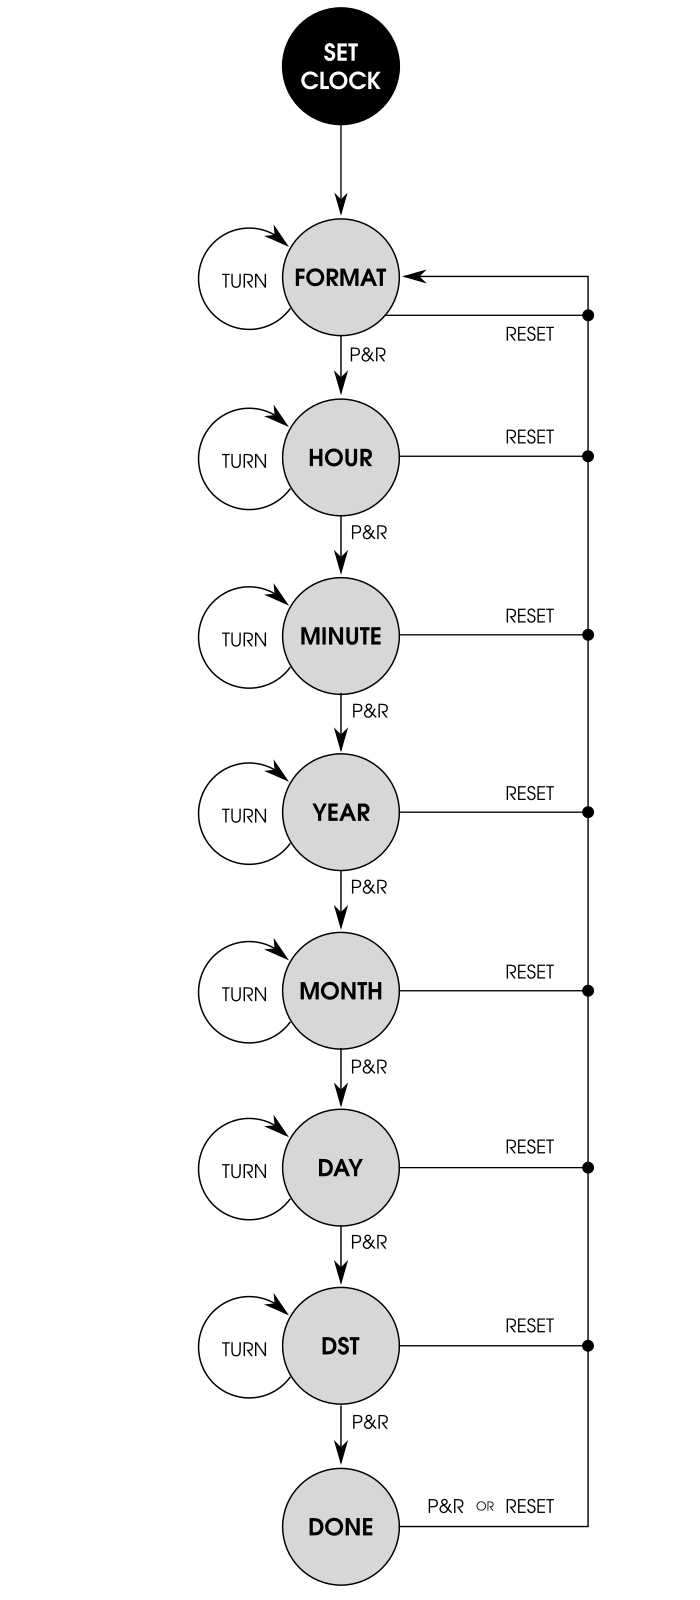
\includegraphics{images/set_clock_state_diagram.png}
\caption{Set Clock - State Diagram} 
\end{figure}
